\chapter{Grundlagen}
\label{cha:grundlagen}

% Abschnitt: Quartettspiel
\section{Quartettspiel}
\label{sec:grundlagen:quartettspiel}

Zum Quartettspielen sind natürlich einige Regeln notwendig, die im Folgenden erklärt werden. \\
Gespielt wird Eins gegen Eins, Spieler gegen Computer. Zuerst wählt der Spieler den Schwierigkeitsgrad (leicht, mittel oder schwer) des Computers, dann den Spielmodus und das Limit für das Spielende (Zeit-, Runden- oder Punktemodus und entsprechend die Spielzeit, Runden- oder Punkteanzahl). Danach wird ein Deck gewählt, gemischt, Computer und Spieler bekommen jeweils die Hälfte der Karten verdeckt auf einem Stapel, bei dem immer nur die oberste Karte sichtbar ist und es wird zufällig bestimmt wer mit dem ersten Zug beginnen darf. Ein Zug sieht immer folgendermaßen aus: Der Spieler, der am Zug ist, wählt ein Attribut (Beispiel: in einem Autoquartett die max. Geschwindigkeit) und nennt den entsprechenden Wert. Der andere Spieler nennt nun ebenfalls seinen Wert (Beispiel von oben: max. Geschwindigkeit) und die Werte werden verglichen. Für jedes Attribut wurde vor einem Spiel festgelegt ob für dieses ein höherer oder niedrigerer Wert gewinnt. Der Vergleich wird also durchgeführt. Der Spieler mit dem besseren Wert gewinnt den Vergleich, bekommt beide Karten der Runde unter seinen Stapel und darf im nächsten Vergleich das Attribut wählen. Bei einem Unentschieden behält jeder seine Karten, legt sie unter seinen Stapel und der Spieler, der das Attribut gewählt hat, wählt auch das Nächste. Das Spiel ist zu Ende, wenn entweder ein Spieler keine Karten mehr auf seinem Stapel hat oder das Limit des gewählten Spielmodus erreicht ist (Zeit abgelaufen, alle Runden ausgespielt oder Punktelimit erreicht).

Dies sind die normalen Regeln und Spielmodi für ein Quartettspiel. In unserer App gibt es aber zusätzlich neben dem normalen Modus (bei dem jeweils, wie festgelegt, der höhere oder niedrigere Wert den Vergleich gewinnt) auch noch den sog. Insanemodus, bei dem jeweils nicht der vorher festgelegte höhere oder niedrigere Wert gewinnt, sondern genau umgekehrt. Damit es im Spiel aber nicht zu Verwirrungen kommt ist immer neben jedem Attribut ein Pfeil, der angibt, ob höher oder niedriger besser ist. 
Egal ob der normale Modus oder Insanemodus gewählt wird, kann man sich noch zusätzlich entscheiden, ob man den Expertenmodus spielen möchte oder nicht. Der Expertenmodus ist aber nichts für Anfänger, denn es werden die Werte einer Karte durch '?' ersetzt, sodass man das Deck bzw. die Karten schon ein bisschen besser kennen muss um hier erfolgreich zu sein.


% Abschnitt: Mobile Plattform
\section{Mobile Plattform}
\label{sec:grundlagen:plattforml}

Android ist ein mobiles Betriebssystem, also für Smartphones und Tablets, das von Google entwickelt wurde und auf Linux basiert. Die App-Entwicklung ist geprägt durch einzelne Aktivitäten (ein angezeigter Screen ist eine Aktivität), die miteinander kommunizieren und in ihrer 'Lebenszeit' ein vorgegebenes Zustandmodell \ref{figure:androidZustandsmodell} durchlaufen.

\begin{figure}[htp]
	\centering
  	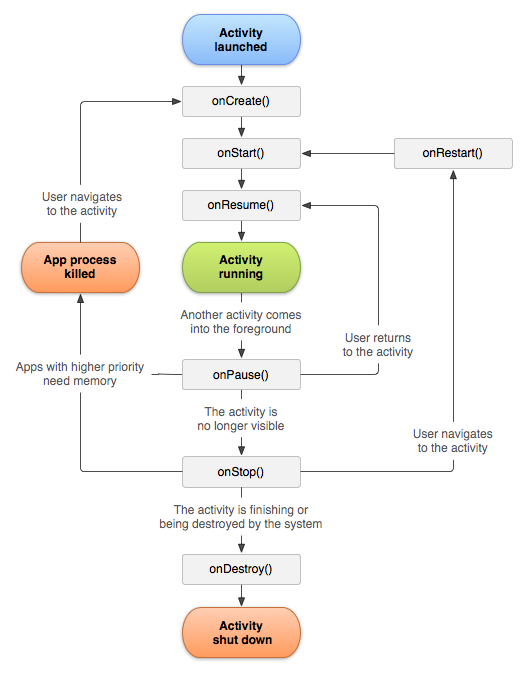
\includegraphics[width=0.33\textwidth]{img/modelle/AndroidZustandsmodell.png}
	\caption[Android Zustandsmodell]{Android Zustandsmodell\protect\footnotemark}
	\label{figure:androidZustandsmodell}
\end{figure}
\footnotetext{http://www.javatpoint.com/images/androidimages/Android-Activity-Lifecycle.png}

Dieses Zustandmodell ist auch anfangs einer der Nachteile von Android, da es nicht so leicht zu verstehen ist und uns auch ein paar Probleme bereitet hat. Nachdem wir uns aber im Laufe der App-Entwicklung immer mehr mit Android vertraut gemacht haben, war auch das Modell kein Problem mehr, sondern eher ein Vorteil, da es sehr logisch und durchdacht ist. Eine weitere Schwierigkeit, die während der Entwicklung aufgetreten ist, ist, dass es so viele verschiedene Android-Versionen und Geräte gibt. Da wir unsere App für so viele Versionen wie möglichen entwickeln wollten, kamen deshalb auch mal das ein oder andere Problem auf, wie z. B. dass manche Libraries oder Frameworks erst ab bestimmten Versionen verfügbar sind oder die vielen verschiedenen Geräte alle unterschiedlichen Seiten- und Größenverhältnisse haben.\\
Die Vorteile von Android überwiegen aber auf jeden Fall, vor allem, wenn man sich damit tiefer beschäftigt und eingearbeitet hat. Einer der größten Vorteile ist die sehr gute Dokumentation von Android durch die das Einlesen in die Möglichkeiten und Funktionen recht leicht ist. Auch die weltweite Verbreitung und Beliebtheit von Android ist hier ein Vorteil, da es sehr viele Entwickler gibt und so jedes Problem schon eimal aufgetreten ist und daher auch zu den allermeisten auch Lösungen oder Workarounds bekannt sind.
Außerdem wird Android stetig Weiterentwickelt, weshalb immer mehr möglich ist und der Umgang mit bestimmten Funktionen, wie z. B. der Zugriff auf Gerätefunktionen wie Kamera oder Galerie immer leichter wird.
Weitere Vorteile für uns sind die Vertrautheit mit Java und die Einfachheit von Android Studio.

% Abschnitt: Frameworks
\section{Frameworks}
\label{sec:grundlagen:frameworks}
Frameworks sind eine Art Gerüst oder Rahmen, die eingesetzt werden um das Programmieren zu vereinfachen und die geschriebenen Zeilen zu verringern.\\
Wir haben in unserer App drei Frameworks als Hilfen genutzt:
\begin{itemize}
\item Picasso\footnote{http://square.github.io/picasso/}: Erlaubt einfaches Handling (z. B. Größentransformationen) von Bildern in oftmals einer Zeile
\item MPAndroidCharts\footnote{https://github.com/PhilJay/MPAndroidChart}: Ermöglicht die Erstellung von Diagrammen (in unserem Fall Tortendiagramme für die Statistiken)
\item Floating Action Button\footnote{https://github.com/Clans/FloatingActionButton}: Ein fancy Menü, das schön ein- und ausgeklappt werden kann
\end{itemize}



















